%% ====================================================================
%% Package management
%% ====================================================================

\section{Package management}

\begin{frame}{Package managers install software without admin rights}
\begin{columns}[c]
    \column{0.62\textwidth}
    Installing tools yourself is hard:
    \begin{itemize}
        \item No admin rights on the HPC, so no \texttt{sudo apt install}
        \item Tools need specific versions of other software, which conflict with each other
        \item ``It works on my computer'' is not reproducible
    \end{itemize}
    \medskip
    Conda solves this:
    \begin{itemize}
        \item Installs in your own directory
        \item Resolves dependencies for you
        \item Separate environments per project
    \end{itemize}
    \column{0.38\textwidth}
    \centering
    
\includegraphics[height=2.2cm]{logo/condaforge.png}\\[0.2cm]
    
\includegraphics[width=0.95\linewidth]{logo/bioconda.png}
\end{columns}
\end{frame}

\begin{frame}{Conda: packages, environments and channels}
\centering\small
\begin{tabular}{@{}lp{0.68\textwidth}@{}}
    \toprule
    \textbf{Term} & \textbf{What it means}                                              \\
    \midrule
    Package       & A tool plus everything it needs, built for one system,
    e.g.\ \texttt{seqkit} for Linux                                                     \\
    Environment   & An isolated folder with a set of packages. Activate it to use them;
    other environments are not affected                                                 \\
    Channel       & An online repository of packages, e.g.\ conda-forge or Bioconda     \\
    Solver        & Works out which versions of all packages fit together               \\
    \bottomrule
\end{tabular}
\end{frame}

\begin{frame}[fragile]{Conda-forge and Bioconda are preferred over defaults}
\small
\begin{itemize}
    \item \textbf{conda-forge}: community channel with general software (Python, R, compilers, \ldots)
    \item \textbf{Bioconda}: bioinformatics tools, builds on top of conda-forge.
          R packages from Bioconductor are here as \texttt{bioconductor-<name>}
    \item \textbf{defaults}: Anaconda's own channel.
          Licence restrictions, and mixing it with conda-forge breaks environments
\end{itemize}
Set this up once:
\begin{lstlisting}
conda config --add channels bioconda
conda config --add channels conda-forge
conda config --set channel_priority strict
\end{lstlisting}
\end{frame}

\begin{frame}[fragile]{Install Miniforge, not Anaconda}
\centering\footnotesize
\begin{tabularx}{\textwidth}{@{}l>{\raggedright\arraybackslash}Xll@{}}
    \toprule
    \textbf{Installer}  & \textbf{Includes}           & \textbf{Channel}     & \textbf{Licence}           \\
    \midrule
    Anaconda            & conda + ready-made packages & defaults             & Paid if $\geq$ 200 staff   \\
    Miniconda3          & conda                       & defaults             & Paid if $\geq$ 200 staff   \\
    \textbf{Miniforge3} & \textbf{conda + mamba}      & \textbf{conda-forge} & \textbf{Open source, free} \\
    \bottomrule
\end{tabularx}

\vspace{0.2cm}
\raggedright\footnotesize
\textbf{Mamba} is a C++ reimplementation of Conda that was much faster.
Since 2023 Conda uses Mamba's solver (\texttt{conda-libmamba-solver}) by default, so \texttt{conda} and \texttt{mamba} now behave almost the same.

\medskip
Install Miniforge: copy the two lines for your laptop
\begin{lstlisting}[basicstyle=\ttfamily\scriptsize]
# Mac (Apple Silicon)
curl -LO https://github.com/conda-forge/miniforge/releases/\
latest/download/Miniforge3-Darwin-arm64.sh
bash Miniforge3-Darwin-arm64.sh

# Linux
curl -LO https://github.com/conda-forge/miniforge/releases/\
latest/download/Miniforge3-Linux-x86_64.sh
bash Miniforge3-Linux-x86_64.sh
\end{lstlisting}
\end{frame}

\begin{frame}[fragile]{The basic Conda workflow}
\begin{lstlisting}
conda create -n qc seqkit   # new env with seqkit
conda activate qc           # start using it
conda install fastp         # add more packages
conda list                  # what is installed here?
conda deactivate            # stop using it

conda env list              # all your environments
conda env remove -n qc      # delete an environment
\end{lstlisting}
\end{frame}

\begin{frame}[fragile]{Your system architecture matters when installing packages}
\small
\begin{itemize}
    \item x86\_64 (Intel, AMD) vs ARM (Apple Silicon: M1 and newer)
    \item Packages are built per system, and some Bioconda packages only exist for x86\_64
    \item The HPC and most Linux laptops are x86\_64, so this only affects Apple Silicon Macs
\end{itemize}
Package not found on your Mac?
Use the x86\_64 version through Rosetta 2:
\begin{lstlisting}
softwareupdate --install-rosetta     # once
CONDA_SUBDIR=osx-64 conda create -n <env> <pkg>
conda activate <env>
conda config --env --set subdir osx-64
\end{lstlisting}
\end{frame}

\begin{frame}[fragile]{Conda on the HPC}
\small
\begin{itemize}
    \item Environments are large: keep them out of your home directory, or you will hit its quota
    \item Install and run tools on a compute node, not on the login node (\texttt{srun}, later today)
\end{itemize}
\begin{lstlisting}[basicstyle=\ttfamily\footnotesize]
conda config --add envs_dirs /hpc/<group>/<user>/conda/envs
conda config --add pkgs_dirs /hpc/<group>/<user>/conda/pkgs
\end{lstlisting}
\end{frame}

\begin{frame}[fragile]{Try it: install a tool with Conda}
\small
\begin{enumerate}
    \item Set up the channels as on the channels slide
    \item Create an environment called \texttt{qc} with \texttt{seqkit}, and activate it
    \item In \texttt{exercise\_data}, run \texttt{seqkit stats} on all assemblies.
          Does \texttt{num\_seqs} match your answers with \texttt{grep -c}?
    \item Deactivate the environment and list all your environments
    \item Bonus: export your environment and push it to your fork
\end{enumerate}
\begin{lstlisting}
seqkit stats */assembly.fasta
conda env export --no-builds > environment.yml
\end{lstlisting}
    {\footnotesize \texttt{>} saves the output of a command to a file}
\end{frame}

\begin{frame}[fragile]{Lock files are much better than Conda env exports!}
\begin{columns}[T]
    \column{0.48\textwidth}
    \small\texttt{environment.yml}
    \begin{lstlisting}[basicstyle=\ttfamily\scriptsize]
channels:
  - conda-forge
  - bioconda
dependencies:
  - seqkit=2.14.0
\end{lstlisting}
    \footnotesize
    \begin{itemize}
        \item Versions, but solved again on install
        \item Result can differ per day and per system
    \end{itemize}
    \column{0.48\textwidth}
    \small\texttt{pixi.lock} {\footnotesize (shortened, made with Pixi: see the extra slide at the end)}
    \begin{lstlisting}[basicstyle=\ttfamily\scriptsize]
- conda: .../bioconda/linux-64/
    seqkit-2.14.0-hb192632_0.conda
  sha256: bd686974e40f8e2c...
  md5: e9381a1fb56f6b73...
\end{lstlisting}
    \footnotesize
    \begin{itemize}
        \item Exact file of every (sub-)dependency
        \item Checksums, for every platform you add
        \item No solving: faster, and identical every time
    \end{itemize}
\end{columns}
\end{frame}

\begin{frame}[fragile]{Containers package the whole system, not just your tools}
\begin{columns}[c]
    \column{0.7\textwidth}
    \small
    \begin{itemize}
        \item A container holds the tool, its dependencies \emph{and} the operating system: it runs the same everywhere
        \item On the HPC use \textbf{Apptainer}: Docker needs admin rights
        \item Apptainer runs Docker images
        \item \textbf{BioContainers}: every Bioconda package automatically gets a container
    \end{itemize}
    \column{0.28\textwidth}
    \centering
    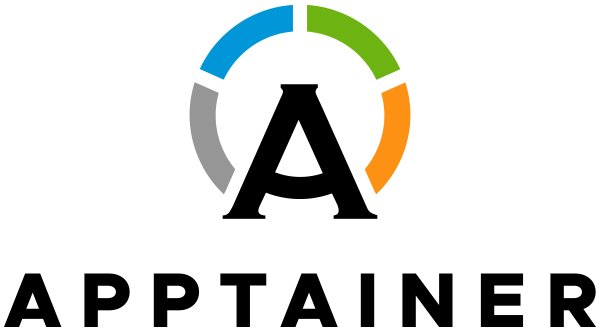
\includegraphics[height=1.3cm]{logo/apptainer.png}\\[0.3cm]
    
\includegraphics[width=0.9\linewidth]{logo/docker.png}
\end{columns}
\begin{lstlisting}[basicstyle=\ttfamily\footnotesize]
apptainer pull \
    docker://quay.io/biocontainers/seqkit:2.14.0--hb192632_0
apptainer exec seqkit_2.14.0--hb192632_0.sif \
    seqkit stats assembly.fasta
\end{lstlisting}
\end{frame}
